%!TEX program = xelatex
\documentclass[aspectratio=169]{beamer}

\usepackage{blindtext}

\usetheme{Execushares}

\title{Structured Sparsity in\\Numerical Optimisation}
\subtitle{Universit\'{e} C\^ote D'Azur, Inria, France}
\author{Matteo Frigo}
\date{Nice - December 4, 2017}

\setcounter{showSlideNumbers}{1}

\usepackage{amsmath,amssymb,amsfonts,amsthm}

%\theoremstyle{definition}
%\newtheorem{problem}{Problem}
%\newtheorem{definition}{Definition}
%\newtheorem{eg}{Example}
%
%\theoremstyle{plain} 
%\newtheorem{theorem}{Theorem}
%\newtheorem{proposition}{Proposition}
%\newtheorem{lemma}{Lemma}
%\newtheorem{property}{Property}
%\newtheorem{corollary}{Corollary}
%\newtheorem{algo}{Algorithm}

\DeclareMathOperator{\Prox}{prox}
\newcommand{\prox}[2]{\Prox_{#1}\left({#2}\right)}

\newcommand{\HH}{\mathcal{H}}
\newcommand{\NN}{\mathbb{N}}
\newcommand{\ZZ}{\mathbb{Z}}
\newcommand{\QQ}{\mathbb{Q}}
\newcommand{\RR}{\mathbb{R}}
\newcommand{\rd}{\mathbb{R}^d}
\newcommand{\CC}{\mathbb{C}}
\newcommand{\norm}[1]{\left\|#1\right\|}
\newcommand{\normtwosq}[1]{\left\|#1\right\|_2^2}
\newcommand{\onehalf}{\frac{1}{2}}
\newcommand {\matlab} {$\text{Matlab}^{\circledR}$\,}
\newcommand {\expect} {\mathbb{E}}
\newcommand {\prob} {\mathbb{P}}
\renewcommand{\epsilon}{\varepsilon}
%\renewcommand{\theta}{\vartheta}
%\renewcommand{\rho}{\varrho}
\renewcommand{\phi}{\varphi}
\hyphenation{sub-dif-fe-ren-tial}
\hyphenation{COMMIT}

\DeclareMathOperator*{\argmin}{argmin}
\DeclareMathOperator{\dom}{dom}

\begin{document}
	\setcounter{showProgressBar}{0}
	\setcounter{showSlideNumbers}{0}

	\frame{\titlepage}
	
	\begin{frame}
	\frametitle{}
	\begin{minipage}{.45\textwidth}
	\begin{center}
	
\includegraphics[height=1cm,keepaspectratio]{img/logo_inria}\\ \quad \\
	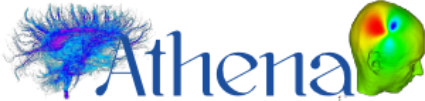
\includegraphics[height=1cm,keepaspectratio]{img/athena-logo}\\ \quad \\
	
\includegraphics[height=1cm,keepaspectratio]{img/flag_yellow_high}\qquad
	
\includegraphics[height=1cm,keepaspectratio]{img/erc_logo}
	\end{center}
	\end{minipage}
	\quad
	\begin{minipage}{.45\textwidth}
	\begin{itemize}
	\item PhD Student
	\item Supervisor: Prof. Rachid Deriche
	\item Inria - Athena Project Team
	\item ERC Computational Brain Connectivity Mapping 
	\item EDSTIC
	\end{itemize}
	\end{minipage}
	\end{frame}
	
	\begin{frame}
		\frametitle{Contents}
		\begin{enumerate}
			\item Mathematics \\ \textcolor{ExecusharesGrey}{\footnotesize\hspace{1em} Proximal Operator, FISTA, Regularisation}
			\item Model Design  \\ \textcolor{ExecusharesGrey}{\footnotesize\hspace{1em} Sparsity, Hierarchy, Lasso}
			\item Brain Imaging \\ \textcolor{ExecusharesGrey}{\footnotesize\hspace{1em} Tractography, dMRI, Connectomics}
		\end{enumerate}
	\end{frame}

	\setcounter{framenumber}{0}
	\setcounter{showProgressBar}{1}
	\setcounter{showSlideNumbers}{1}
	\section{Mathematics}
		
		\begin{frame}
			\frametitle{Numerical Optimisation}
			\quad \\
			\begin{itemize}
			\item $\HH$ is a set
			\item $\Phi: \HH\to\RR$
			\item Find \begin{equation}\nonumber x^* = \argmin_{x\in\HH}\Phi(x)\end{equation}
			\end{itemize}
			
%			\pause
%			\vfill
			
%			Our setting:
%			\begin{itemize}
%			\item $\HH=\rd$
%			\item $\Phi(x) := f(x) + g(x)$
%				\begin{itemize}
%				\item $f(x)$ is convex and has $L$-Lipschitz continuous gradient
%				\item $g(x)$ is convex and lower semi-continuous
%				\end{itemize}
%			\item Find \begin{equation}\nonumber x\in\rd = \argmin_{x\in\rd}f(x)+g(x)\end{equation}
%			\end{itemize}
			
		\end{frame}

		\begin{frame}
			\frametitle{Smooth case}
			\begin{minipage}{.45\textwidth}
			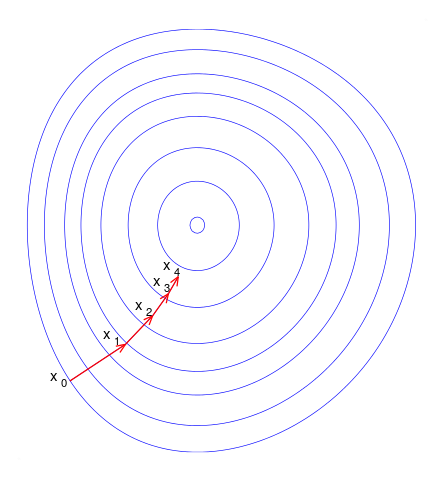
\includegraphics[width=\textwidth]{img/gradientdescent}
			\end{minipage}\qquad
			\begin{minipage}{.45\textwidth}
			Smooth case: $g(x) = 0$
			\begin{equation}\nonumber
			x^*=\argmin_{x\in\rd}f(x).
			\end{equation}
			Iteration:
			\begin{equation}
			\nonumber
			x^+ = x - \gamma\nabla f(x)
			\end{equation}
			with $\gamma=\frac{1}{L}$
			\end{minipage}
		\end{frame}

		\begin{frame}
		\frametitle{Non-smooth case}
		Let $\{C_j\}_j$ sequence of cvx subsets of $\rd$ with non-empty intersection,
		\begin{equation}
		\nonumber
		x^*=\argmin_{x\in \rd}\sum_j \iota_{C_j}(c)
		\end{equation}
		\pause
		POCS: Projection Onto Convex Sets
		\begin{equation}
		\nonumber
		x_{k+1} = \Pi_{C_1}\Pi_{C_2}\cdots\Pi_{C_N} x_k.
		\end{equation}
		\pause
		Each projection is the solution of 
		\begin{equation}
		\nonumber
		\argmin_{y\in \rd}\frac{1}{2}\normtwosq{x-y} + \iota_{C_j}(y).
		\end{equation}
		\end{frame}
		
		\begin{frame}
		\frametitle{Proximal operator}
		$\Gamma_0(\mathcal{H}) = \left\{f:\mathcal{H}\to\RR\text{ l.s.c. and cvx with } \dom(f)\ne\emptyset\right\}$
		\quad \\ \quad \\
		\begin{definition}[Proximal Operator]
		\label{def:proximaloperator}
		Let $f\in\Gamma_0(\RR^N)$. For every $x \in \RR^N$, the minimisation problem
		\begin{equation}
		\nonumber
		\argmin_{y\in\RR^N} f(y) + \frac{1}{2}\normtwosq{x-y}
		\end{equation}
		admits a unique solution which is called as $\prox{f}{x}$.
		\end{definition}
		\end{frame}

		\begin{frame}
		\frametitle{Properties of $\Prox$}
		{Separability}:
		\begin{equation}
		\nonumber f(x,y) = \phi(x)+\psi(y) = \prox{\phi}{x} + \prox{\psi}{y}
		\end{equation}
		
		{Nonexpansiveness}:
		\begin{equation}
		\nonumber \normtwosq{\prox{f}{x}-\prox{f}{y}} \le \left(x-y\right)^T\left(\prox{f}{x} - \prox{f}{y}\right)
		\end{equation}
		
		{Resolvent operator}: 
		\begin{equation}
		\nonumber \prox{f}{\cdot} = \left(I + \partial f\right)^{-1} (\cdot)
		\end{equation}
		\end{frame}
		
		\begin{frame}
		\frametitle{Properties of $\Prox$: part 2}
		The convex conjugate of $f:X\to\RR$ is $f^*:X^*\to\RR$
		\begin{equation}
		\nonumber
		f^*(\xi) = \sup_{x\in X}\left<\xi,x\right>-f(x)
		\end{equation}
		\pause
		{Moreau decomposition}:
		\begin{gather}
		\nonumber v = \prox{f}{v} + \prox{f^*}{v}\\
		\nonumber v = \Pi_L(v) + \Pi_{L^\perp}(v)\\
		\nonumber v = \Pi_K(v) + \Pi_{K^\circ}(v)
		\end{gather}
		\begin{proof}
		$2+2=4-1=3$ quick mafhs.
		\end{proof}
		\end{frame}
		
		\begin{frame}
		\frametitle{$Prox$ of norms}
		Consider $f = \|\cdot\|$ and $\mathcal{B} = \left\{x : \norm{x}_*\le 1 \right\}$, then
		\begin{equation}
		\nonumber f^* \left(\xi\right) = \iota_{C_j}\mathcal{B}\left(\xi\right)
		\end{equation}
		
		By Moreau decomposition:
		\begin{gather}
		\nonumber v = \prox{f}{v} + \Pi_{\mathcal{B}}(v)\\
		\nonumber \prox{\norm{\cdot}}{v} = v - \Pi_{\mathcal{B}}(v)
		\end{gather}
		\pause
		\begin{center}
		\textbf{We have the proximal operator of norms!}
		\end{center}
		\end{frame}
		
		\begin{frame}
		\frametitle{Key property}
		A point $x^*\in \RR^n$ is a minimiser of $f$ if and only if 
		\begin{equation}
		\label{eq:fixedpointprox}
		\prox{f}{x^*} = x^*.
		\end{equation}
		\end{frame}
		
		\begin{frame}
		\frametitle{Greedy algorithm}
		Objective: minimise $f$, for which we can compute $\Prox_f$\\
		\begin{itemize}
		\pause\item $\Prox$ is firmly non-expansive
		\pause\item The minimiser $x^*$ is a fixed point of $\Prox$
		\end{itemize}
		\pause
		Iteration:
		\begin{equation}\nonumber
		x_{k+1} = \prox{f}{x_k}
		\end{equation}
		
		\pause
		If we don't know anything about the Lipschitz constant of $\Prox_f$
		\begin{equation}
		\nonumber x_{k+1} = [(1-\alpha)I + \alpha\Prox_f](x_k)
		\end{equation}
		\quad \\
		\begin{center}
		\textcolor{ExecusharesGrey}{\tiny Cominetti et al., On the rate of convergence of Krasnoselskii-Mann iterations and their connection with	sums of Bernoullis, 2014}
		\end{center}
		\end{frame}
		
		\begin{frame}
		\frametitle{Interpretation}
		Gradient descent of the Moreau envelope
		\begin{equation}
		\nonumber M_{f} = \left(f^* + (1/2)\normtwosq{\cdot}\right)^*
		\end{equation}
		\pause \textbf{NB:} the minimisers of $f$ and $M_f$ coincide
		\end{frame}
		
		
\end{document}